\documentclass{beamer}

\usepackage[T1]{fontenc}
\usepackage[utf8]{inputenc}
\usepackage[spanish]{babel}
\usepackage{lmodern}
\usepackage{algorithmic, algorithm, listings , tikz }
\usetikzlibrary{ arrows.meta }

\usetikzlibrary{shapes.geometric, arrows, positioning}



\definecolor{nubankpurple}{RGB}{130, 10, 209} % El morado de Nubank
\definecolor{lambdaorange}{RGB}{255, 140, 0}

\definecolor{codegreen}{rgb}{0,0.6,0}
\definecolor{codegray}{rgb}{0.5,0.5,0.5}
\definecolor{codepurple}{rgb}{0.58,0,0.82}
\definecolor{backcolour}{rgb}{ 150 , 150 , 150 }
\definecolor{handwriting}{rgb}{0.6, 0.2, 0.2}

\lstset{
    language=Java,
    backgroundcolor=\color{backcolour},   
    commentstyle=\color{codegreen},
    keywordstyle=\color{magenta},
    numberstyle=\tiny\color{codegray},
    stringstyle=\color{codepurple},
    basicstyle=\ttfamily\scriptsize,
    breakatwhitespace=false,         
    breaklines=true,                 
    captionpos=b,                    
    keepspaces=true,                 
    showspaces=false,                
    showstringspaces=false,
    showtabs=false,                  
    tabsize=2
}

% Use Unipd as theme, with options:
% - pageofpages: define the separation symbol of the footer page of pages (e.g.: of, di, /, default: of)
% - logo: position another logo near the Unipd logo in the title page (e.g. department logo), passing the second logo path as option 
% Use the environment lastframe to add the endframe text

\usetheme[pageofpages=of]{Unipd}

\title{Sesión 1: Programación Funcional }
\subtitle{  Semillero en Ciencias de la Computación }
\author[Ostos, Pedrozo ]{Joel Ostos \and Juan Pedrozo}

\date{ Abril 24, 2026 }

% The next block of commands puts the table of contents at the beginning of each section and highlights the current section
\AtBeginSection[]
{
  \begin{frame}
    \frametitle{Tabla de Contenidos }
    \tableofcontents[currentsection]
  \end{frame}
}

\begin{document}

\frame{\titlepage}

\begin{frame}{ Tabla de contenidos }
    \tableofcontents    
\end{frame}

\section{ Un vistazo a la programación funcional y sus alrededores }

\subsection{Paradigmas de programación}
\begin{frame}{Paradigmas de programación }
    \begin{enumerate}
        \item Orientado a Objetos.
        \item Imperativo.
        \item Declarativo.
        \item Funcional.
    \end{enumerate}
\end{frame}
\subsubsection{POO}
\begin{frame}{ Programación Orientada a Objetos }
    Antes, la programación era mayormente procedural. Los programas eran una larga lista de instrucciones.
    POO tiene como pilares:
    \begin{enumerate}
        \item Encapsulamiento
        \item Abstracción
        \item Herencia
        \item Polimorfismo
    \end{enumerate}
\end{frame}
\begin{frame}{Encapsulamiento}
    Agrupar datos y comportamiento en una sola unidad: el \textbf{objeto}.
    \begin{itemize}
        \item El objeto expone solo lo necesario
        \item El resto queda \textit{oculto} al exterior
    \end{itemize}
    \vspace{0.5em}
    \texttt{persona.nombre} \quad vs \quad \texttt{persona.\_id\_interno}
\end{frame}

\begin{frame}{Abstracción}
    Modelar el mundo real ignorando los detalles irrelevantes.
    \begin{itemize}
        \item Un \texttt{Auto} tiene \texttt{acelerar()} — no importa cómo funciona el motor
        \item Se trabaja con \textit{qué hace}, no \textit{cómo lo hace}
    \end{itemize}
\end{frame}

\begin{frame}{Herencia}
    Una clase puede \textit{heredar} atributos y métodos de otra.
    \begin{itemize}
        \item \texttt{Perro} y \texttt{Gato} heredan de \texttt{Animal}
        \item Favorece la reutilización de código
    \end{itemize}
    \vspace{0.5em}
    \texttt{Animal} $\rightarrow$ \texttt{Perro}, \texttt{Gato}, \texttt{Ave} \ldots
\end{frame}

\begin{frame}{Polimorfismo}
    El mismo mensaje, distintos comportamientos según el objeto.
    \begin{itemize}
        \item \texttt{animal.hablar()} $\rightarrow$ \textit{"Guau"} o \textit{"Miau"} según sea el caso
        \item El código no necesita saber \textit{qué tipo} de objeto es
    \end{itemize}
\end{frame}
\subsubsection{Programación Imperativa}
\begin{frame}[fragile]
    \frametitle{Programación Imperativa }

    \begin{lstlisting}
    public static int calculateScore(String word) {
        int score = 0;
        for(char c : word.toCharArray()) {
            score++;
        }
        return score;
    }
    \end{lstlisting}
    \vspace{0.5cm}
    \small
    La programación imperativa se enfoca en el \textbf{como} debe ser computado el resultado.

\end{frame}

\subsubsection{Programación Declarativa}
\begin{frame}[fragile]
    \frametitle{Programación Declarativa }

    \begin{lstlisting}
    public static int wordScore(String word) {
        return word.length();
    }
    \end{lstlisting}
    \vspace{0.5cm}
    \small
    La programación declarativa se enfoca en qué se necesita hacer, no como.\\
    Generalmente es más sencilla de leer que la programación imperativa.
\end{frame}

\begin{frame}{Dos visiones de la computación}
    \begin{columns}
        \begin{column}{0.45\textwidth}
            \centering
            \textbf{Alan Turing} \\
            \vspace{0.3em}
            Máquina de estados, instrucciones secuenciales \\
            \vspace{0.3em}
            \small $\rightarrow$ Programación \textbf{Imperativa}
        \end{column}
        \begin{column}{0.45\textwidth}
            \centering
            \textbf{Alonzo Church} \\
            \vspace{0.3em}
            Cálculo Lambda, transformación de funciones \\
            \vspace{0.3em}
            \small $\rightarrow$ Programación \textbf{Funcional}
        \end{column}
    \end{columns}
    \vspace{0.8em}
    \begin{alertblock}{}
        \centering
        \small Ambos modelos son equivalentes en poder computacional, pero proponen \textit{maneras distintas de pensar}.
    \end{alertblock}
\end{frame}

\begin{frame}{Máquina de Turing: ¿Es $0^n1^n$?}
\begin{center}
\begin{tikzpicture}[
    >=Stealth,
    every node/.style={font=\scriptsize},
    st/.style={circle, draw, thick, minimum size=0.85cm},
    ac/.style={circle, draw, double, thick, minimum size=0.85cm},
]
    \node[st] (q0) at (0,0)    {$q_0$};
    \node[st] (q1) at (3.5,0)  {$q_1$};
    \node[st] (q2) at (7,0)    {$q_2$};
    \node[st] (q3) at (0,-3)   {$q_3$};
    \node[ac] (qa) at (3.5,-3) {$q_{acc}$};

    % Flecha inicial
    \draw[->] (-1,0) -- (q0);

    % q0 -> q1
    \draw[->] (q0) -- node[below]{$0 \to A,\;R$} (q1);

    % q1 -> q2
    \draw[->] (q1) -- node[below]{$1 \to B,\;L$} (q2);

    % q2 -> q0 (arco por arriba)
\draw[->] (q2) to[out=150, in=30] node[above]{$A \to A,\;R$} (q0);

    % q0 -> q3
    \draw[->] (q0) -- node[left]{$B \to B,\;R$} (q3);

    % q1 loop
    \draw[->] (q1) to[loop below] node[align=center]{
        $0 \to 0,\;R$\\$B \to B,\;R$} (q1);

    % q2 loop
    \draw[->] (q2) to[loop below] node[align=center]{
        $B \to B,\;L$\\$0 \to 0,\;L$} (q2);

    % q3 loop
    \draw[->] (q3) to[loop below] node{$B \to B,\;R$} (q3);

    % q3 -> qacc
    \draw[->] (q3) -- node[above]{$\sqcup \to \sqcup,\;R$} (qa);

\end{tikzpicture}
\end{center}
\end{frame}

\begin{frame}[fragile]{El mismo problema en Cálculo Lambda}
\begin{verbatim}
(defn count-ady [s]
  (->> (partition-by identity s) 
       (map (juxt first count))))

(defn fmt-ady [s]
  (let [coll (count-ady s)]
      (when (= (count coll) 2)
       (let [[[_ n1] [_ n2]] coll]
         (= n1 n2)))))
\end{verbatim}

\vspace{0.4em}
\begin{alertblock}{Diferencia fundamental}
\small La MT \textit{recorre} una cinta modificando símbolos paso a paso.
El cálculo lambda \textbf{transforma} la lista con funciones — sin mutación, sin estados.
\end{alertblock}
\end{frame}

\subsubsection{Cálculo Lambda}
\begin{frame}[fragile]{El Origen: Cálculo Lambda ($\lambda$)}
    \begin{itemize}
        \item \textbf{¿Qué es?}: Un sistema matemático formal para expresar la computación basado en la \textbf{abstracción de funciones}.
        \item \textbf{Influencia}: Es la base teórica de todos los lenguajes funcionales (Lisp, Haskell, Clojure).
    \end{itemize}

    \begin{exampleblock}{Los tres pilares del Cálculo Lambda}
        \begin{enumerate}
            \item \textbf{Variables}: $x$
            \item \textbf{Abstracción}: $\lambda x . M$ (Define una función que toma $x$ y devuelve $M$)
            \item \textbf{Aplicación}: $(M \, N)$ (Aplica la función $M$ al argumento $N$)
        \end{enumerate}
    \end{exampleblock}

    \vspace{0.3cm}
    \begin{center}
        \textit{En Clojure, una función anónima \texttt{(fn [x] (* x x))} es una abstracción lambda.}
    \end{center}
\end{frame}

\subsection{Un poco de historia}
\begin{frame}{Un poco de historia}
    \centering
    \begin{tikzpicture}[node distance=1.2cm, every node/.style={font=\tiny, align=center}]

        % Línea central
        \draw[gray!50, line width=2pt, ->] (0,0) -- (10.5,0);

        % --- HITOS ---

        % 1930s - Cálculo Lambda
        \filldraw[lambdaorange] (0.5,0) circle (3pt);
        \node[above=0.2cm of {(0.5,0)}] (lambda) {\textbf{1936}\\[-1pt]Cálculo Lambda\\(Alonzo Church)};
        \node[below=0.2cm of {(0.5,0)}, text width=1.5cm, gray] {Fundamento matemático de la PF.};

        % 1958 - LISP
        \filldraw[blue!70] (2.5,0) circle (3pt);
        \node[above=0.2cm of {(2.5,0)}] (lisp) {\textbf{1958}\\[-1pt]LISP\\(John McCarthy)};
        \node[below=0.2cm of {(2.5,0)}, text width=1.5cm, gray] {Primer lenguaje funcional práctico.};

        % 1990 - Haskell
        \filldraw[purple!80] (4.5,0) circle (3pt);
        \node[above=0.2cm of {(4.5,0)}] (haskell) {\textbf{1990}\\[-1pt]Haskell\\(Estándar)};
        \node[below=0.2cm of {(4.5,0)}, text width=1.8cm, gray] {PF pura y tipado estático fuerte.};

        % 2007 - Clojure
        \filldraw[green!60!black] (6.5,0) circle (3pt);
        \node[above=0.2cm of {(6.5,0)}] (clojure) {\textbf{2007}\\[-1pt]Clojure\\(Rich Hickey)};
        \node[below=0.2cm of {(6.5,0)}, text width=1.8cm, gray] {Lisp moderno sobre la JVM.};

        % 2013 - Nubank
        \filldraw[nubankpurple] (8.5,0) circle (3pt);
        \node[above=0.2cm of {(8.5,0)}] (nu) {\textbf{2013}\\[-1pt]Fundación de\\Nubank};
        \node[below=0.2cm of {(8.5,0)}, text width=1.8cm, gray] {Adopción masiva de Clojure en FinTech.};

        % 2020 - Adquisición Cognitect
        \filldraw[red!70!black] (10.2,0) circle (4pt);
        \node[above=0.2cm of {(10.2,0)}, color=red!70!black] (acq) {\textbf{2020}\\[-1pt]Adquisición de\\Cognitect};
        \node[below=0.2cm of {(10.2,0)}, text width=2cm, gray] {Nubank adquiere a los creadores de Clojure.};

    \end{tikzpicture}

    \vspace{0.5cm}
    \begin{block}{Dato relevante}
        \scriptsize
        Gracias al cálculo lambda se puede demostrar que algún lenguaje es turing completo, como lo es el caso de Clojure y Haskell.
    \end{block}
\end{frame}

\subsection{Qué es la programación Funcional}
\begin{frame}[fragile]
    \frametitle{ Entonces, ¿Qué es la programación funcional? }
    \begin{center}
        Programación mediante \textbf{transformaciones}, no mediante órdenes.
    \end{center}
    \begin{enumerate}
        \item \textbf{Cero efectos secundarios (Side Effects) }
        \item \textbf{Inmutabilidad }
        \item \textbf{Funciones Puras }
    \end{enumerate}
\end{frame}

\subsubsection{Efectos secundarios}
\begin{frame}[fragile]
    \frametitle{ ¿Qué son los efectos secundarios? }
    Cuando el único resultado observable de una función es el valor que retorna decimos que la función no tiene efectos secundarios. \\
    Si su función cambia alguna variable global o local más allá del valor que retorna entonces esta posee efectos secundarios.
    \begin{lstlisting}
    public class EjemploSideEffect {

        static int contador = 0;

        public static void foo( ) {
            contador++; // side effect
        }

        public static void main(String[] args) {
            foo();
            System.out.println(contador);
        }
    }
    \end{lstlisting}
\end{frame}

\subsubsection{Inmutabilidad}

\begin{frame}[fragile]
    \frametitle{Inmutabilidad}
    \begin{enumerate}
    \item Los datos no cambian después de crearse.
    \item En lugar de modificar un valor se crea uno nuevo
    \item Hace que el comportamiento del código sea más predecible pues se evitan los \textbf{side effects} 
    \end{enumerate}
\end{frame}

\subsubsection{Funciones Puras}
\begin{frame}[fragile]
    \frametitle{Funciones Puras}

    \begin{minipage}{0.5\textwidth}
        \begin{enumerate}
            \item Misma entrada $\rightarrow$ Misma salida.
            \item No tienen efectos secundarios.
            \item Son predecibles y fáciles de probar.
        \end{enumerate}
        \end{minipage}
    \begin{minipage}{0.4\textwidth}
        \begin{lstlisting}[language=Java]
int suma(int a, int b) {
        return a + b;
}
        \end{lstlisting}
    \end{minipage}
\end{frame}





\begin{frame}[fragile]
    \frametitle{¿Qué tan útil es aprender programación funcional? }
    \begin{enumerate}
        \item Es un estilo de escribir código en cualquier lenguaje.
        \item Es como un cambio de chip en la manera de pensar en programación declarativa.
    \end{enumerate}
    \begin{figure}
        \centering
        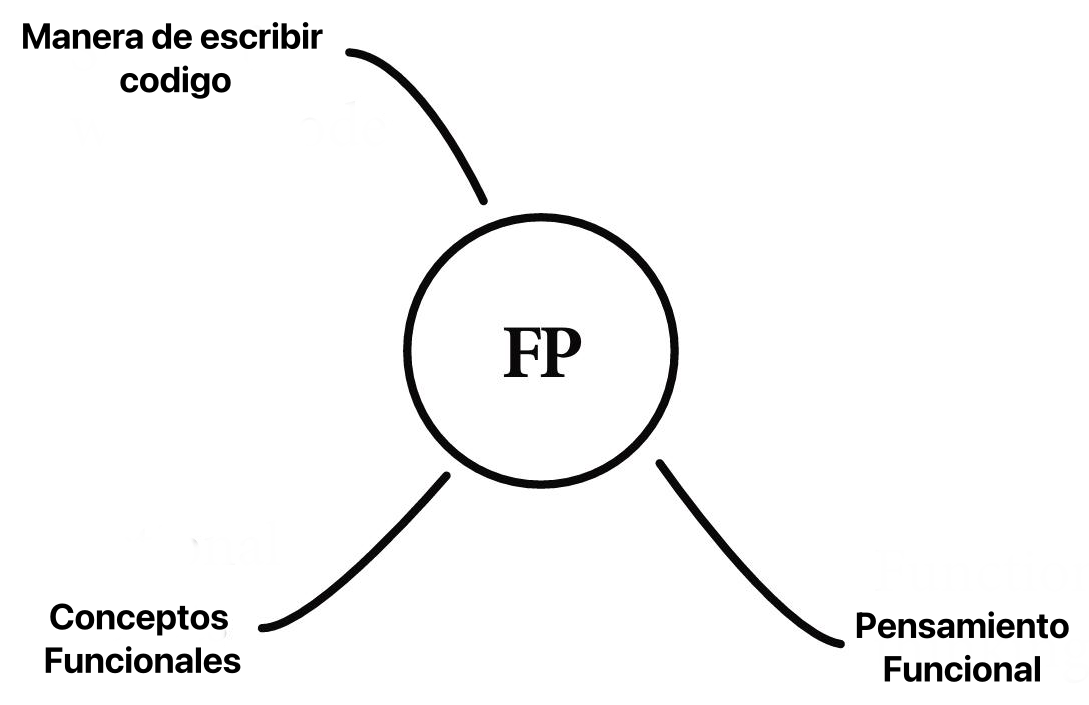
\includegraphics[width=0.6\linewidth]{figs/fp1.png}
    \end{figure}
\end{frame}

\section{Ejemplos Prácticos en Clojure}

\begin{emptyframe}
    Aplicación en Clojure
\end{emptyframe}

\begin{frame}
    \frametitle{¿Qué es Clojure?}
    \begin{itemize}
        \item \textbf{Lisp:} Dialecto potente y expresivo con un enfoque funcional puro.
        \item \textbf{Alojado:} Diseñado para ejecutarse sobre plataformas existentes.
        \begin{itemize}
            \item Principalmente la \textbf{JVM} (Java Virtual Machine).
            \item También compila a JavaScript y CLR (.NET).
        \end{itemize}
    \end{itemize}

    \vspace{0.5cm}

    \begin{block}{Compilación en la JVM}
        El compilador (\texttt{clojure.jar}) transforma el código fuente directamente en \textbf{Java Bytecode}, aprovechando el recolector de basura y el manejo de hilos de Java.
    \end{block}

    \vspace{0.5cm}
\end{frame}

\begin{frame}[fragile]{¿Qué es Lisp?}
    \begin{itemize}
        \item \textbf{LISt Processing}
        \item \textbf{Homoiconicidad:} Código igual que estructuras de datos
        \item \textbf{Prefix notation}
    \end{itemize}

    \begin{exampleblock}{Anatomía de una Expresión}
        \begin{itemize}
            \item Estructura: \texttt{(operador argumento1 argumento2 ...)}
        \end{itemize}
        \begin{center}
        \begin{verbatim}
        ;; Suma simple: (+ 1 2 3) -> 6
        
        (defn saludar [nombre]
          (str "Hola, " nombre))
        \end{verbatim}
        \end{center}
    \end{exampleblock}

\end{frame}

\begin{frame}{El Proceso de Evaluación}
    \begin{columns}
        \begin{column}{0.5\textwidth}
            \begin{enumerate}
                \item \textbf{Reader:} Texto a estructuras de datos
                \item \textbf{Data Structures} 
                \item \textbf{Evaluator} 
                \item \textbf{Result} 
            \end{enumerate}
        \end{column}
        
        \begin{column}{0.45\textwidth}
            \begin{figure}
                \centering
                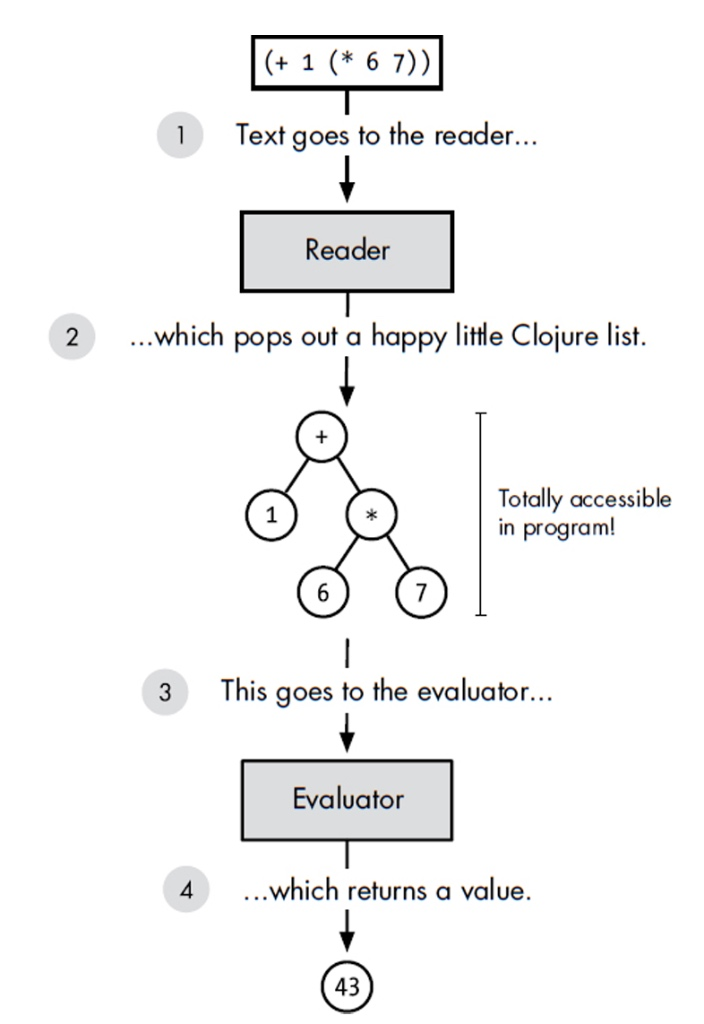
\includegraphics[width=\textwidth]{eval.jpeg} 
            \end{figure}
        \end{column}
    \end{columns}
\end{frame}

\begin{frame}{Funciones Anidadas}
    \begin{columns}
    \begin{column}{0.5\textwidth}
            \begin{enumerate}
                \item Las funciones anidadas se leen de paréntesis interiores a exteriores
            \end{enumerate}
        \end{column}
        \begin{column}{0.65\textwidth}
            \begin{figure}
                \centering
                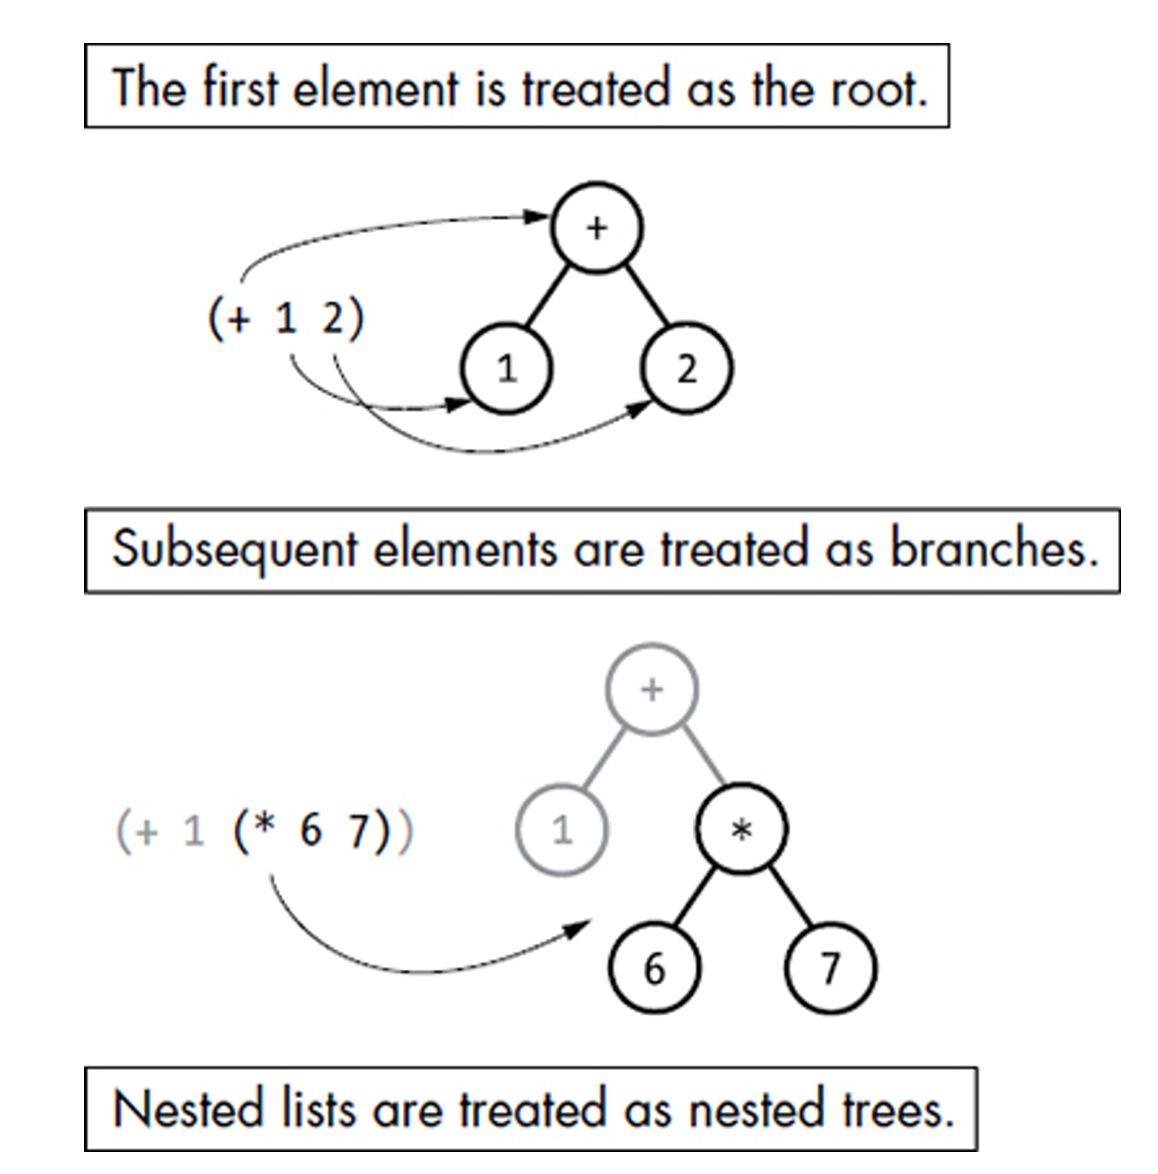
\includegraphics[width=\textwidth]{nested.jpeg} 
            \end{figure}
        \end{column}
    \end{columns}
\end{frame}

\begin{frame}[fragile]{Definición de Funciones}
    \begin{itemize}
        \item Se utiliza la macro \texttt{defn}.
        \item Los parámetros se definen dentro de un \textbf{vector} \texttt{[]}.
        \item El cuerpo de la función devuelve automáticamente el valor de la última expresión.
    \end{itemize}

    \begin{exampleblock}{Sintaxis Básica}
        \begin{verbatim}
        (defn saludar []
          (println "Hola Mundo"))

        (defn calcular-area [radio]
          (* 3.14 (* radio radio)))

        (defn promedio [a b]
          (/ (+ a b) 2))
        \end{verbatim}
    \end{exampleblock}
\end{frame}

\begin{frame}[fragile]{El REPL: Desarrollo Interactivo}
    \begin{itemize}
        \item \textbf{¿Qué es?}: \textit{Read-Eval-Print Loop}. Una interfaz para interactuar con un proceso de Clojure en ejecución.
        \item \textbf{Filosofía}: Permite modificar el programa en vivo incluso en producción, similar a una conexión SSH.
        \item \textbf{Feedback Inmediato}: Ideal para experimentar con sintaxis y lógica sin reiniciar la aplicación.
    \end{itemize}

\end{frame}

\begin{frame}[fragile]{Ejemplo de Interacción}
        \begin{exampleblock}{Uso del REPL}
        \begin{verbatim}
        user=> (+ 1 2 3 4)
        10

        user=> (first [1 2 3 4])
        1

        (do 
          (println "Evaluando...")
          (+ 1 3))
        ; => Evaluando...
        4
        \end{verbatim}
    \end{exampleblock}
\end{frame}

\begin{frame}[fragile]{println como side effect}

    \begin{exampleblock}{El caso de \texttt{println}}
        \begin{verbatim}

        user=> (println "Hola semillero!")
        ; Hola semillero! <--- SIDE EFFECT 
        nil <--- VALOR DE RETORNO
        
        \end{verbatim}
    \end{exampleblock}

    \begin{alertblock}{¿Por qué es un Side Effect?}
        Porque \texttt{println} no devuelve el texto; su trabajo es \textbf{modificar el estado de la pantalla}. En Clojure, \texttt{println} siempre devuelve \texttt{nil} como valor.
    \end{alertblock}
\end{frame}

\begin{frame}{Recursos: ¡A practicar Clojure!}
    \begin{itemize}
        \item \textbf{4Clojure (Interactive Problems):} La mejor plataforma para aprender la sintaxis y el pensamiento funcional mediante retos progresivos.
        \item \textbf{¿Qué encontrarás?}: Desde cómo funcionan las listas hasta la manipulación avanzada de datos.
    \end{itemize}

    \begin{block}{Ejercicios Interactivos}
        Puedes encontrar y resolver ejemplos prácticos en:
        \vspace{0.3cm}
        \begin{center}
            \href{https://4clojure.oxal.org/}{\textbf{\texttt{https://4clojure.oxal.org/}}}
        \end{center}
    \end{block}
    
\end{frame}

\begin{emptyframe}
    Gracias!
\end{emptyframe}
\end{document}
